In the performance results presented here, a data point is the 
average from $10$ randomly generated \opg instances. All algorithms 
are implemented in Python 2.7, and all experiments are executed on 
an Intel\textsuperscript{\textregistered} Xeon\textsuperscript{\textregistered} 
%E5-1660 v3 
CPU at 3.0GHz. % with 32GB RAM.% at 2133MHz.
Some additional performance results can be found in the Appendix.

%\subsubsection{\algoMRSimple} 
For the case of $m$ perimeters each containing a single segment, for 
each $1 \le i \le m$, we set $len(\partial R_i) = 1$ and let $len(P_i)$ 
be uniformly distributed in $(0, 1]$. ~\ref{fig:opg-mpsc-example} shows 
the result for an example with $m = 10$ and $n = 30$. For various values 
of $m, n$, the running time of \algoMRSimple is summarized in 
Table~\ref{eval:opg-mpsc}, which scales very well with $m$ and $n$ (note that 
the $n \le m$ case does not make much sense here). 

\begin{figure}[ht!]
    \vspace*{-3mm}
    \centering
    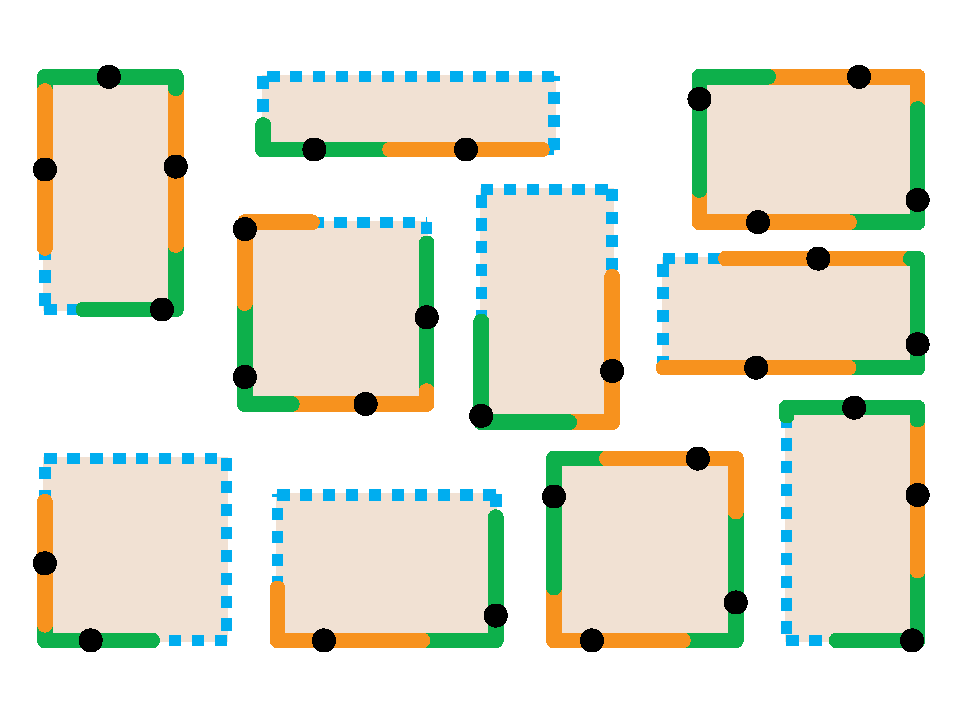
\includegraphics[keepaspectratio, scale=0.32]{./chapters/opg/figures/mpsc-example-eps-converted-to.pdf}
    \vspace*{-6mm}
    \caption[An example problem instance for MPSC]{\label{fig:opg-mpsc-example} 
    An example problem instance when $m = 10$ and $n = 30$. The black dots
		indicate deployed robot locations; the green and orange lines indicate
		the coverage.
    %We use blue dashed lines to show the gaps which do not need to be covered. 
    %The black filled circles illustrate final robot deployment locations, and 
    %the orange/green lines demonstrate individual robot covers. 
    %In this example, we use a different distribution to sample $len(P_i)$ due to 
    %cosmetic reasons.
		}
    \vspace*{-2mm}
\end{figure}

\begin{table}[ht!]
    \centering
		\vspace*{-4mm}
    \begin{footnotesize}
    \begin{tabular}{|c|c|c|c|c|c|c|} 
        \hline
        \diagbox{$m$}{$n$}       & $10^8  $ & $10^9   $ & $10^{10}$ & $10^{11}$ & $10^{12}  $ \\ \hline
        %\rule{0pt}{2.5ex} $10^3$ & $0.001 $ & $0.001  $ & $0.001  $ & $0.001  $ & $0.001    $ \\ \hline
        %\rule{0pt}{2.5ex} $10^4$ & $0.006 $ & $0.007  $ & $0.008  $ & $0.008  $ & $0.008    $ \\ \hline
        %\rule{0pt}{2.5ex} $10^5$ & $0.075 $ & $0.088  $ & $0.102  $ & $0.107  $ & $0.106    $ \\ \hline
        \rule{0pt}{2.5ex} $10^6$ & $1.152 $ & $1.442  $ & $1.508  $ & $1.652  $ & $1.617    $ \\ \hline
        \rule{0pt}{2.5ex} $10^7$ & $13.963$ & $17.281 $ & $18.796 $ & $20.354 $ & $20.627   $ \\ \hline
        \rule{0pt}{2.5ex} $10^8$ & NA       & $176.115$ & $223.186$ & $227.250$ & $230.000  $ \\ \hline
    \end{tabular}
		\end{footnotesize}
		% \vspace*{-3mm}
    \caption{\label{eval:opg-mpsc} \algoMRSimple~running time (seconds)}
		% \vspace*{-4mm}
\end{table}

%Recall that when the problem has multiple perimeters with single components, 
%each perimeter has exactly one segment and at most one gap. Our problem 
%generation procedure works as follows: given the number of perimeters $m$, we 
%first generate $m$ rectangles $\{R_1, \dots, R_m\}$ with $len(\partial R_i) = 1$ 
%for all $1 \leq i \leq m$, and then select a closed connected component $P_i$ 
%for each $R_i$. Here, $len(P_i)$ is uniformly randomly sampled from $(0, 1]$. 
%An example problem instance along with its optimal cover is shown in 
%~\ref{fig:mpsc-example}. The computation time of \algoMRSimple~under 
%different $m$ and $n$ is presented in Table.~\ref{eval:mpsc}. 
%\sh{Plots here. The constant factor in the $O(m(\log n + \log m) + \sum_{i} M_i)$ time 
%complexity is around $5 \times 10^{-8}$ seconds. }

For the case of a single perimeter with multiple components, a random 
polygon is generated on which $2q$ points are randomly sampled that 
yield $q$ segments (that form the perimeter) and $q$ gaps. An example 
instance and the optimal solution with $q=3$ and $n = 10$ is illustrated 
in ~\ref{fig:opg-spmc-example}. The computation time for various $q$ and 
$n$ combinations is given in Table~\ref{eval:opg-spmc}.
\begin{figure}[ht!]
    % \vspace*{-3mm}
    \centering
    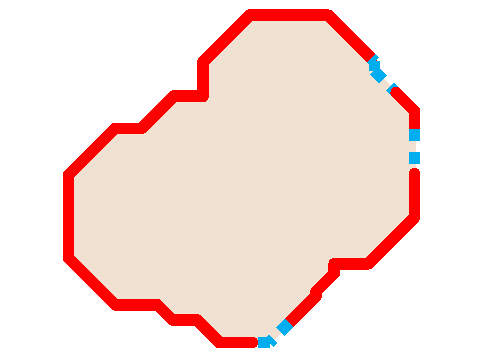
\includegraphics[keepaspectratio, scale=0.4]{./chapters/opg/figures/spmc-example-eps-converted-to.pdf}
    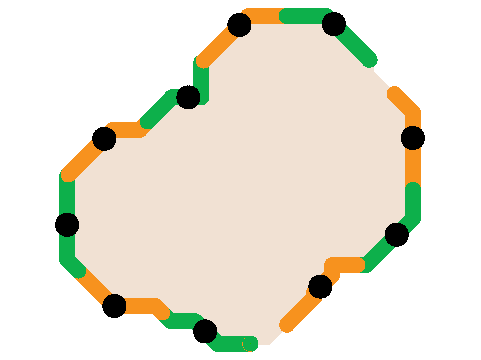
\includegraphics[keepaspectratio, scale=0.4]{./chapters/opg/figures/spmc-solution-eps-converted-to.pdf}
    % \vspace*{-3mm}
    \caption[Example OPG problem instance of SPMC]{\label{fig:opg-spmc-example} 
    An example problem instance when $q = 3$ and $n = 10$. In this case, the 
		optimal cover actually covers one gap.}
    % \vspace*{-4mm}
\end{figure}

\begin{table}[ht!]
    % \vspace*{-3mm}
    \footnotesize
    \centering
    \begin{tabular}{|c|c|c|c|c|c|c|} 
        \hline
        \diagbox{$q$}{$n$}       & $10^1   $ & $10^2   $ & $10^3  $  & $10^4   $ & $10^5$   \\ \hline       
        \rule{0pt}{2.5ex} $10^2$ & $0.013  $ & $0.015  $ & $0.016 $  & $0.016  $ & $0.017$  \\ \hline   
        \rule{0pt}{2.5ex} $10^3$ & $1.363  $ & $1.595  $ & $1.622 $  & $1.634  $ & $1.641$  \\ \hline   
        \rule{0pt}{2.5ex} $10^4$ & $159.404$ & $188.497$ & $210.492$ & $212.473$ & $212.780$\\ \hline   
    \end{tabular}
    \vspace*{-3mm}
    \caption{\label{eval:opg-spmc} \algoSRG~computation time (seconds)}
    \vspace*{-4mm}
\end{table}


%\subsubsection{\algoSRG} 
%To generate a problem of a single perimeter divided by interlaced segments and gaps, 
%we first create an arbitrary polygon $R$. Then, we uniformly randomly sample $2q$ points 
%on $\partial R$ to divide it into $q$ segments and $q$ gaps. 
%An example problem instance along with its optimal cover is shown in 
%~\ref{fig:spmc-example}. The computation time of 
%\algoSRG~under different $q$ and $n$ is presented in Table~\ref{eval:spmc}.

For multiple perimeters containing multiple components, $m$ polygons 
are created with $len(\partial R_i)$ randomly distributed in $[1, 10]$. 
For setting $q_i$, we fix a $q$ and let $q_i = q(0.5 + random(0, 1))$. 
Representative computation results of \algoMRG are listed in 
Table~\ref{eval:opg-mpmc}.
%whose perimeters' lengths are uniformly randomly sampled from interval $(1, 10)$. 
%The computation time under different $m$, $q$, and $n$ values are provided in Table~\ref{eval:mpmc}. 
%We observe that with the same $q$, $n$ parameters, the computation time is directly proportional to $m$.
\begin{table}[ht!]
    \vspace*{-2mm}
    \footnotesize
    \centering
    \begin{tabular}{|c|c|c|c|c|c|c|} 
        \hline
        \multirow{2}{*}{$q$} & \multirow{2}{*}{$n$} & \multicolumn{5}{|c|}{$m$} \\ \cline{3-7}
        \rule{0pt}{2.5ex} & & $10$ & $20$ & $30$ & $40$ & $50$ \\ \hline
        %\rule{0pt}{2.5ex} $10^1$ & $10^2$ & $ 0.015$ & $ 0.027$ & $ 0.039$ & $ 0.045$ & $ 0.054$ \\ \hline
        \rule{0pt}{2.5ex} $10^1$ & $10^3$ & $ 0.047$ & $ 0.063$ & $ 0.076$ & $ 0.091$ & $ 0.108$ \\ \hline
        %\rule{0pt}{2.5ex} $10^2$ & $10^2$ & $ 1.492$ & $ 2.784$ & $ 4.168$ & $ 5.404$ & $ 6.444$ \\ \hline
        \rule{0pt}{2.5ex} $10^2$ & $10^3$ & $ 2.191$ & $ 3.771$ & $ 5.523$ & $ 7.707$ & $ 9.369$ \\ \hline
        \rule{0pt}{2.5ex} $10^2$ & $10^4$ & $ 7.105$ & $ 9.619$ & $11.369$ & $12.760$ & $15.107$ \\ \hline
    \end{tabular}
    \vspace*{-3mm}
    \caption{\label{eval:opg-mpmc} \algoMRG~computation time (seconds)}
    \vspace*{-4mm}
\end{table}

Due to limited space, only selected essential performance data is 
presented here. More complete performance data and associate analysis 
can be found in the Appendix. 

